%%%%%%%%%%%%%%%%%%%%%%%%%%%%%%%%%%%%%%%%%%%%%%%%%%%%%%%%%%%%%%%%%%%%%%%%%%%%%%%%%%%%
% Document data
%%%%%%%%%%%%%%%%%%%%%%%%%%%%%%%%%%%%%%%%%%%%%%%%%%%%%%%%%%%%%%%%%%%%%%%%%%%%%%%%%%%%
\documentclass[12pt]{report} %report allows for chapters
\renewcommand\thesection{\arabic{section}} % ignore the title number for sections
%%%%%%%%%%%%%%%%%%%%%%%%%%%%%%%%%%%%%%%%%%%%%%%%%%%%%%%%%%%%%%%%%%%%%%%%%%%%%%%%%%%%




%%%%%%%%%%%%%%%%%%%%%%%%%%%%%%%%%%%%%%%%%%%%%%%%%%%%%%%%%%%%%%%%%%%%%%%%%%%%%%%%%%%%
% Packages
%%%%%%%%%%%%%%%%%%%%%%%%%%%%%%%%%%%%%%%%%%%%%%%%%%%%%%%%%%%%%%%%%%%%%%%%%%%%%%%%%%%%
\usepackage{color, soul, xcolor} % Colored text and highlighting, respectively

%Tikz
\usepackage{tikz-cd} % For commutative diagrams
\usepackage{tikz-3dplot}
\RequirePackage{pgfplots}
\usetikzlibrary{shadows}
\usetikzlibrary{shapes}
\usetikzlibrary{decorations}
\usetikzlibrary{arrows,decorations.markings} 
\usetikzlibrary{quotes,angles}

\usepackage{mathtools}
\usepackage{answers}
\usepackage{setspace}
\usepackage{graphicx}
\usepackage{enumerate}
\usepackage{multicol}
\usepackage{mathrsfs}
\usepackage[margin=1in]{geometry} 
\usepackage{amsmath,amsthm,amssymb}
\usepackage{marvosym,wasysym} %fucking smileys
\usepackage{float}
\usepackage{morefloats}
%%%%%%%%%%%%%%%%%%%%%%%%%%%%%%%%%%%%%%%%%%%%%%%%%%%%%%%%%%%%%%%%%%%%%%%%%%%%%%%%%%%%




%%%%%%%%%%%%%%%%%%%%%%%%%%%%%%%%%%%%%%%%%%%%%%%%%%%%%%%%%%%%%%%%%%%%%%%%%%%%%%%%%%%%
% Shortcuts
%%%%%%%%%%%%%%%%%%%%%%%%%%%%%%%%%%%%%%%%%%%%%%%%%%%%%%%%%%%%%%%%%%%%%%%%%%%%%%%%%%%%
% Number systems
\newcommand{\N}{\mathbb{N}}
\newcommand{\Z}{\mathbb{Z}}
\newcommand{\C}{\mathbb{C}}
\newcommand{\R}{\mathbb{R}}
\newcommand{\Q}{\mathbb{Q}}

% Operators/functions
\newcommand{\id}{\mathrm{Id}}
\DeclareMathOperator{\sech}{sech}
\DeclareMathOperator{\csch}{csch}
%%%%%%%%%%%%%%%%%%%%%%%%%%%%%%%%%%%%%%%%%%%%%%%%%%%%%%%%%%%%%%%%%%%%%%%%%%%%%%%%%%%%




%%%%%%%%%%%%%%%%%%%%%%%%%%%%%%%%%%%%%%%%%%%%%%%%%%%%%%%%%%%%%%%%%%%%%%%%%%%%%%%%%%%%
% Environments
%%%%%%%%%%%%%%%%%%%%%%%%%%%%%%%%%%%%%%%%%%%%%%%%%%%%%%%%%%%%%%%%%%%%%%%%%%%%%%%%%%%%
% Italic font
\newtheorem{theorem}{Theorem}[section]
\newtheorem{lemma}{Lemma}[section]
\newtheorem{corollary}{Corollary}[section]
\newtheorem{axiom}{Axiom}

% Plain font
\theoremstyle{definition}
\newtheorem{definition}{Definition}[section]
\newtheorem{example}{Example}[section]
\newtheorem{remark}{Remark}[section]
\newtheorem{solution}{Solution}
\newtheorem{problem}{Problem}[section]
\newtheorem{question}{Question}[section]
\newtheorem{answer}{Answer}[section]
\newtheorem{exercise}{Exercise}[section]
%%%%%%%%%%%%%%%%%%%%%%%%%%%%%%%%%%%%%%%%%%%%%%%%%%%%%%%%%%%%%%%%%%%%%%%%%%%%%%%%%%%%

\begin{document}


\begin{center}
   \textsc{\large MATH 255, Homework 7: \emph{Solutions}}\\
\end{center}
\vspace{.5cm}

\noindent\textbf{Problem 1.} Let's examine the idea of level curves and surfaces a bit more.  For all of the functions, will consider levels $c_0 = \frac{1}{2}$, $c_1=1$, $c_2=2$, and $c_3=3$.  
\begin{enumerate}[(a)]
    \item Given the function
    \[
    f(x)=\frac{1}{\|x\|}=\frac{1}{\sqrt{x^2}},
    \]
    plot this.  Then find the \emph{level points} corresponding to $c_0,c_1,c_2,$ and $c_3$.
    \item Given the function
    \[
    g(x,y) = \frac{1}{\|(x,y)\|}=\frac{1}{\sqrt{x^2+y^2}},
    \]
    plot this.  Then find the \emph{level curves} corresponding to $c_0,c_1,c_2,$ and $c_3$.
    \item Given the function,
    \[
    h(x,y,z) = \frac{1}{\|(x,y,z)\|}=\frac{1}{\sqrt{x^2+y^2+z^2}},
    \]
    find the \emph{level surfaces} corresponding to $c_0,c_1,c_2,$ and $c_3$. 
    \emph{Note, I didn't ask you to plot $h$ itself since there is not a nice way to do so.}
\end{enumerate}
What's the point? Most functions we care about deal with $\R^3$.  However, we don't have ways to visualize these functions without the use of level surfaces.  So, working to understand the analogs of level surfaces is key.
\begin{solution}~
\begin{enumerate}[(a)]
    \item We first solve this problem algebraically then we'll deal with the plots.  We have
    \begin{align*}
        f(x)&=c\\
        \iff \frac{1}{\sqrt{x}^2} &= c\\
        \iff \sqrt{x^2}&=\frac{1}{c}\\
        \iff x^2&= \frac{1}{c^2}\\
        \iff x &= \pm \frac{1}{c}.
    \end{align*}
    Now using this, we find that the level points follow:
    \begin{align*}
        \textrm{For $c_0=\frac{1}{2}$:~}\quad x&=\pm 2\\
        \textrm{For $c_1=1$:~}\quad x&=\pm 1\\
        \textrm{For $c_2=2$:~}\quad x&=\pm \frac{1}{2}\\
        \textrm{For $c_3=3$:~}\quad x&=\pm \frac{1}{3}.\\
    \end{align*}
    Here are the plots.
    \begin{figure}[H]
        \centering
        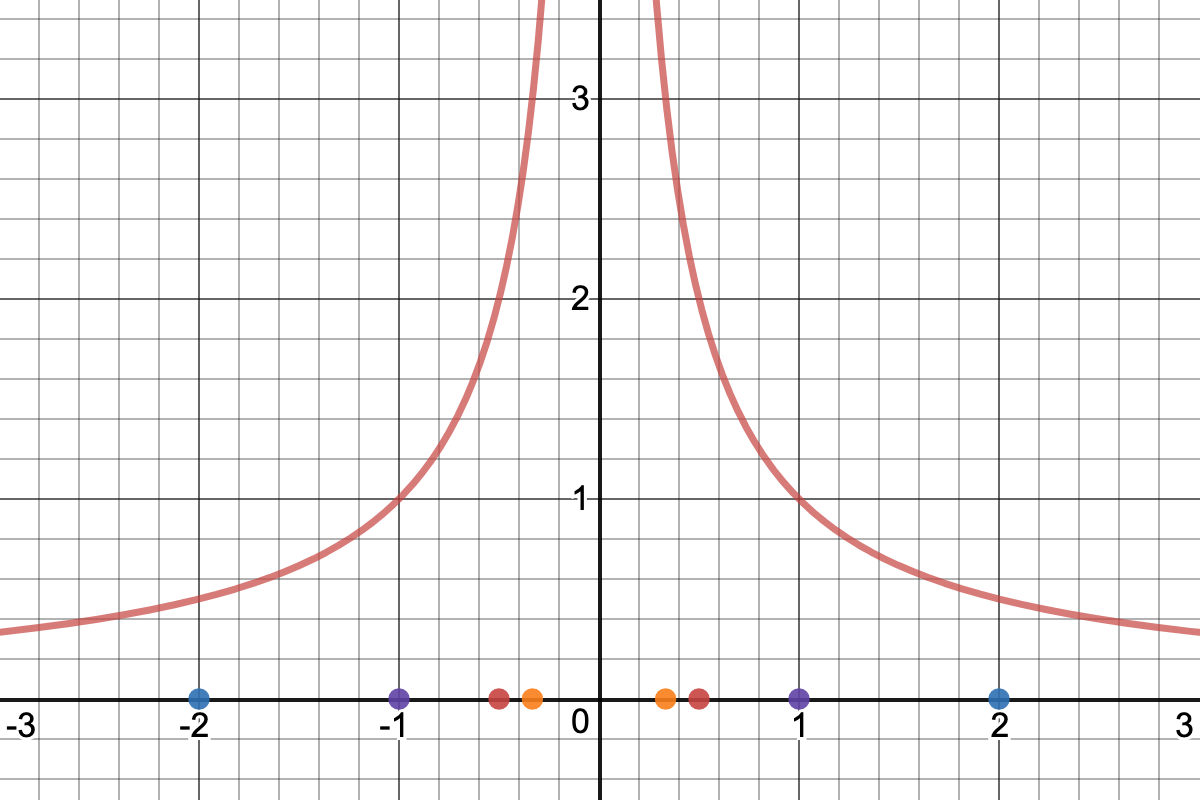
\includegraphics[width=.6\textwidth]{Images/level_points.png}
        \caption{Graph of $f(x)$ with level points on the $x$-axis.}
    \end{figure}
    \item Let's repeat the same process as in (a). We take
    \begin{align*}
        g(x,y)&=c\\
        \iff \frac{1}{\sqrt{x^2+y^2}}&= c\\
        \iff \sqrt{x^2+y^2}&=\frac{1}{c}\\
        \iff x^2+y^2 &= \frac{1}{c^2},
    \end{align*}
    which is the equation for a circle of radius $\frac{1}{c}$. Now using this, we find that the level curves follow:
    \begin{align*}
        \textrm{For $c_0=\frac{1}{2}$:~}\quad x^2+y^2&=2\\
        \textrm{For $c_1=1$:~}\quad x^2+y^2&=1\\
        \textrm{For $c_2=2$:~}\quad x^2+y^2&=\frac{1}{4}\\
        \textrm{For $c_3=3$:~}\quad x^2+y^2&=\frac{1}{9}.\\
    \end{align*}
    Here are the plots.
    \begin{figure}[H]
        \centering
        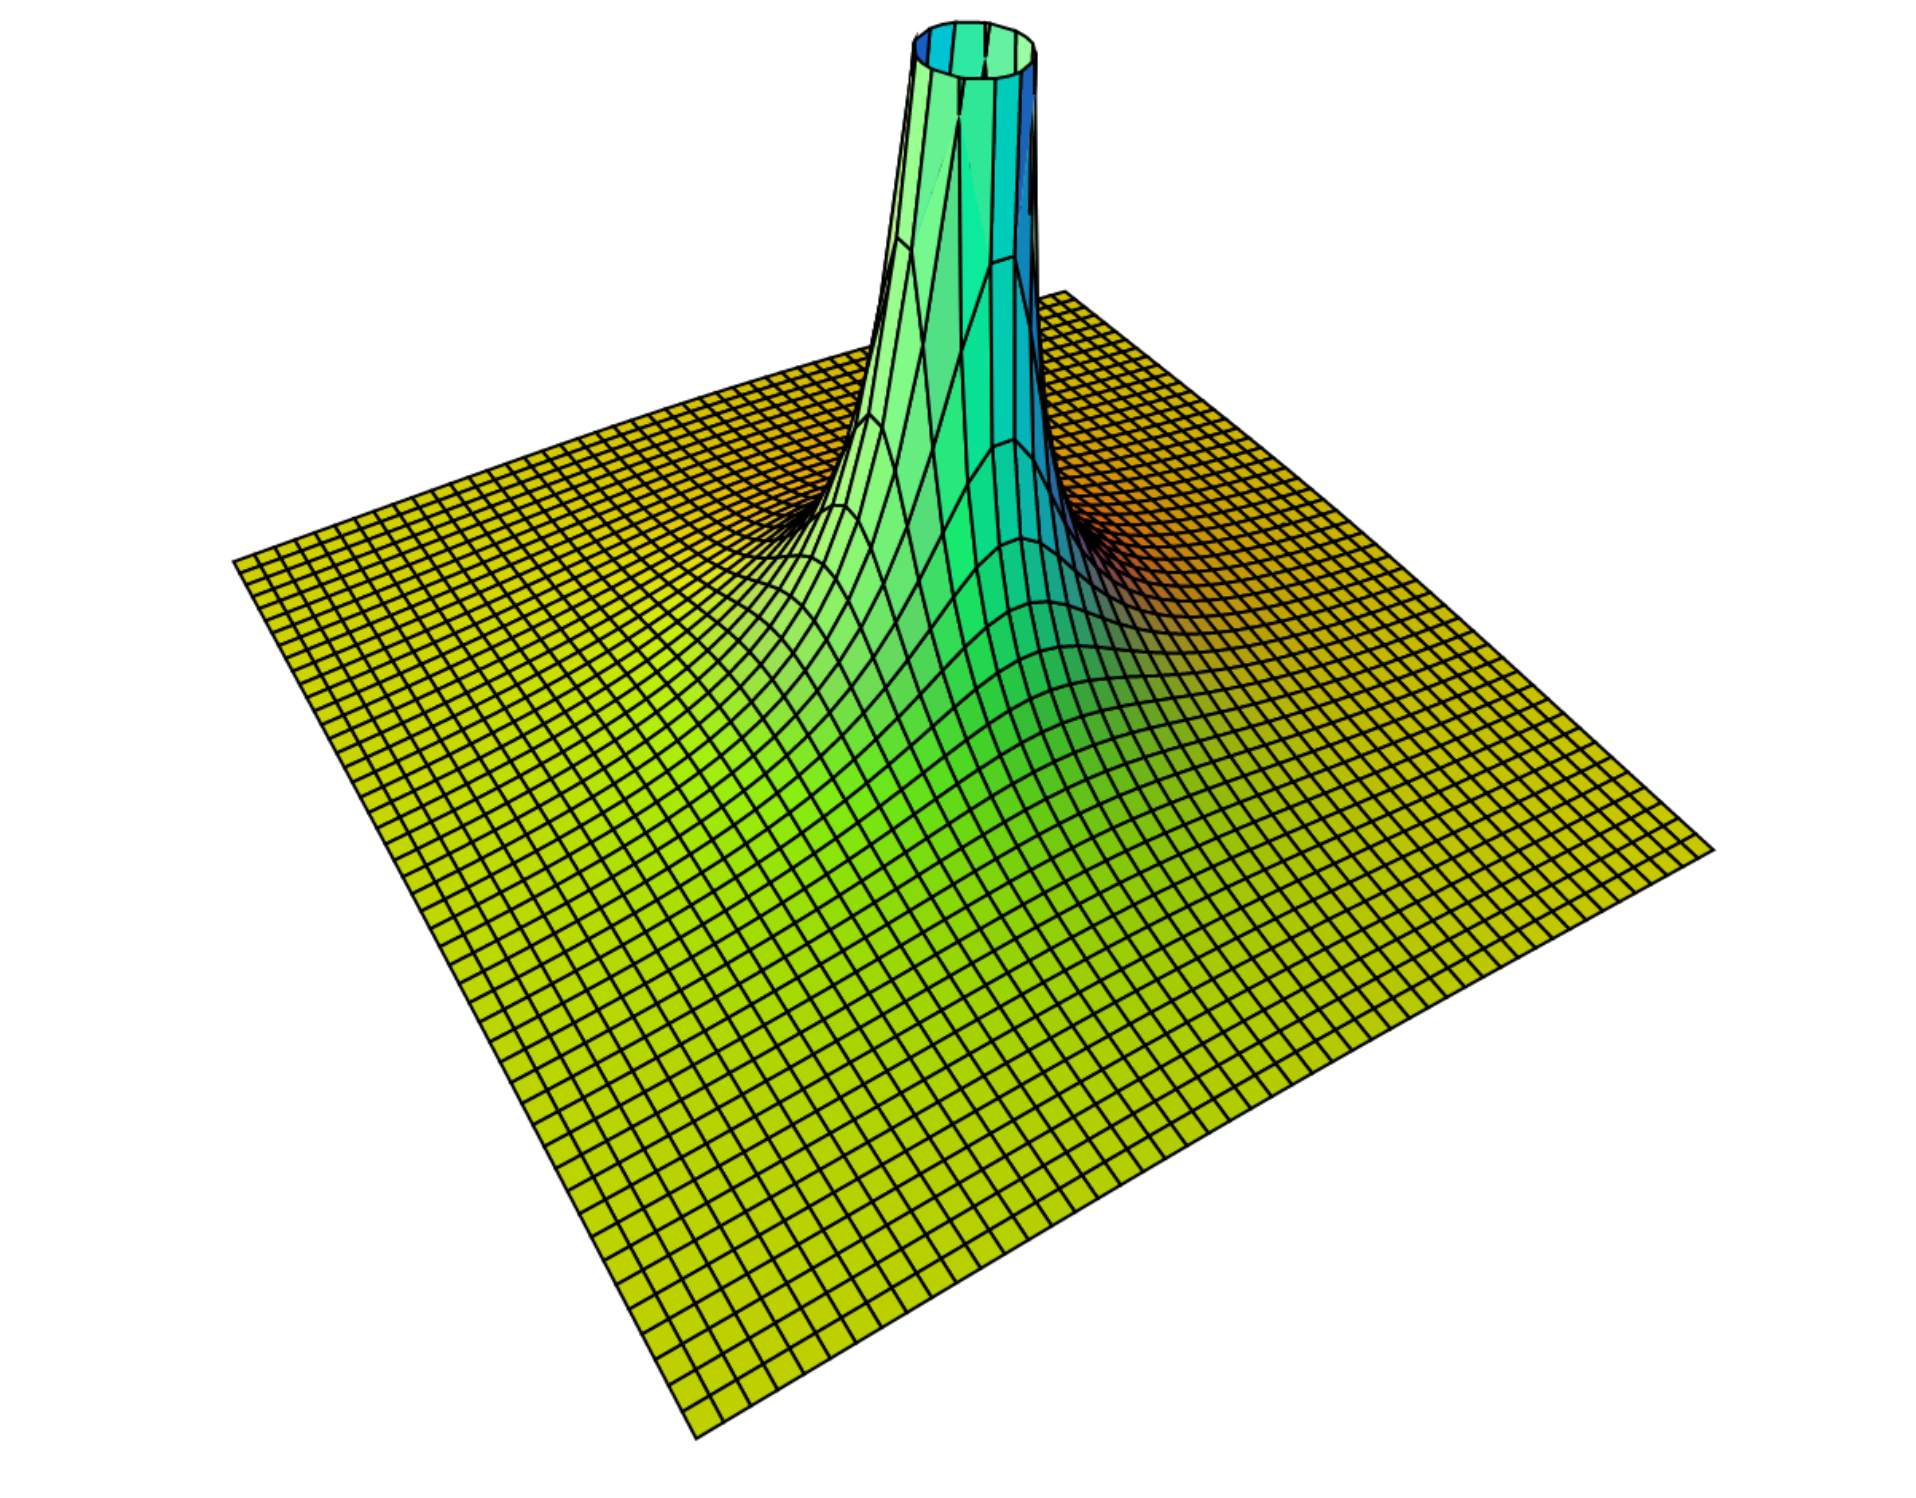
\includegraphics[width=.6\textwidth]{Images/level_curve_surface.png}
        \caption{The graph of the function $g(x,y)$.}
    \end{figure}
    \begin{figure}[H]
        \centering
        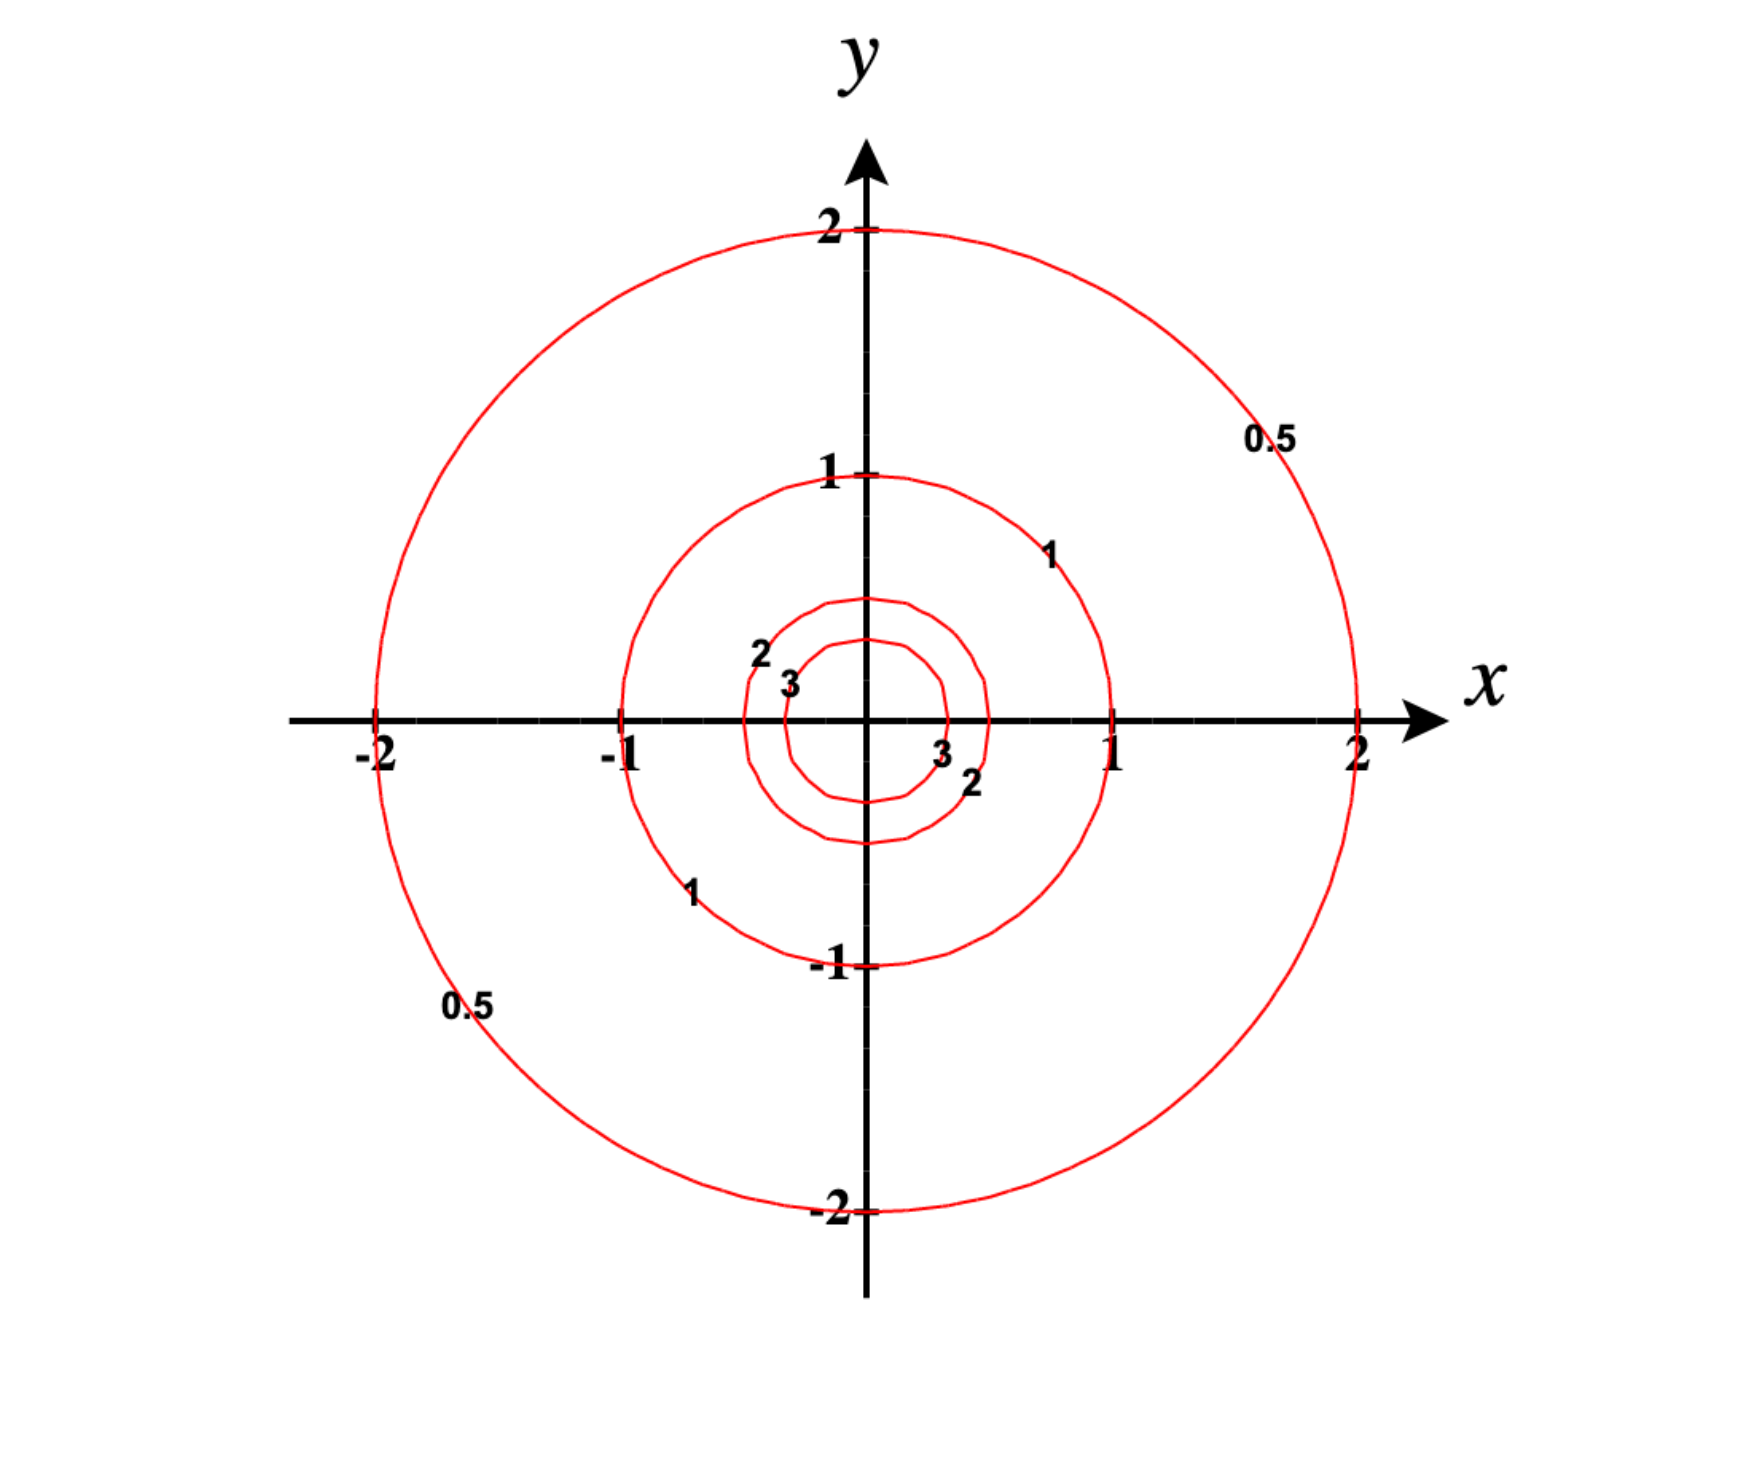
\includegraphics[width=.6\textwidth]{Images/level_curves.png}
        \caption{The level curves for the function $g(x,y)$.}
    \end{figure}
    \item Let's repeat the process one last time, so we have
    \begin{align*}
            h(x,y,z)&=c\\
        \iff \frac{1}{\sqrt{x^2+y^2+z^2}}&= c\\
        \iff \sqrt{x^2+y^2+z^2}&=\frac{1}{c}\\
        \iff x^2+y^2+z^2 &= \frac{1}{c^2},
    \end{align*}
    which is the equation for a sphere of radius $\frac{1}{c}$.  Then the level surfaces follow:
        \begin{align*}
        \textrm{For $c_0=\frac{1}{2}$:~}\quad x^2+y^2+z^2&=2\\
        \textrm{For $c_1=1$:~}\quad x^2+y^2+z^2&=1\\
        \textrm{For $c_2=2$:~}\quad x^2+y^2+z^2&=\frac{1}{4}\\
        \textrm{For $c_3=3$:~}\quad x^2+y^2+z^2&=\frac{1}{9}.\\
    \end{align*}
    Here are the plots
    \begin{figure}[H]
        \centering
        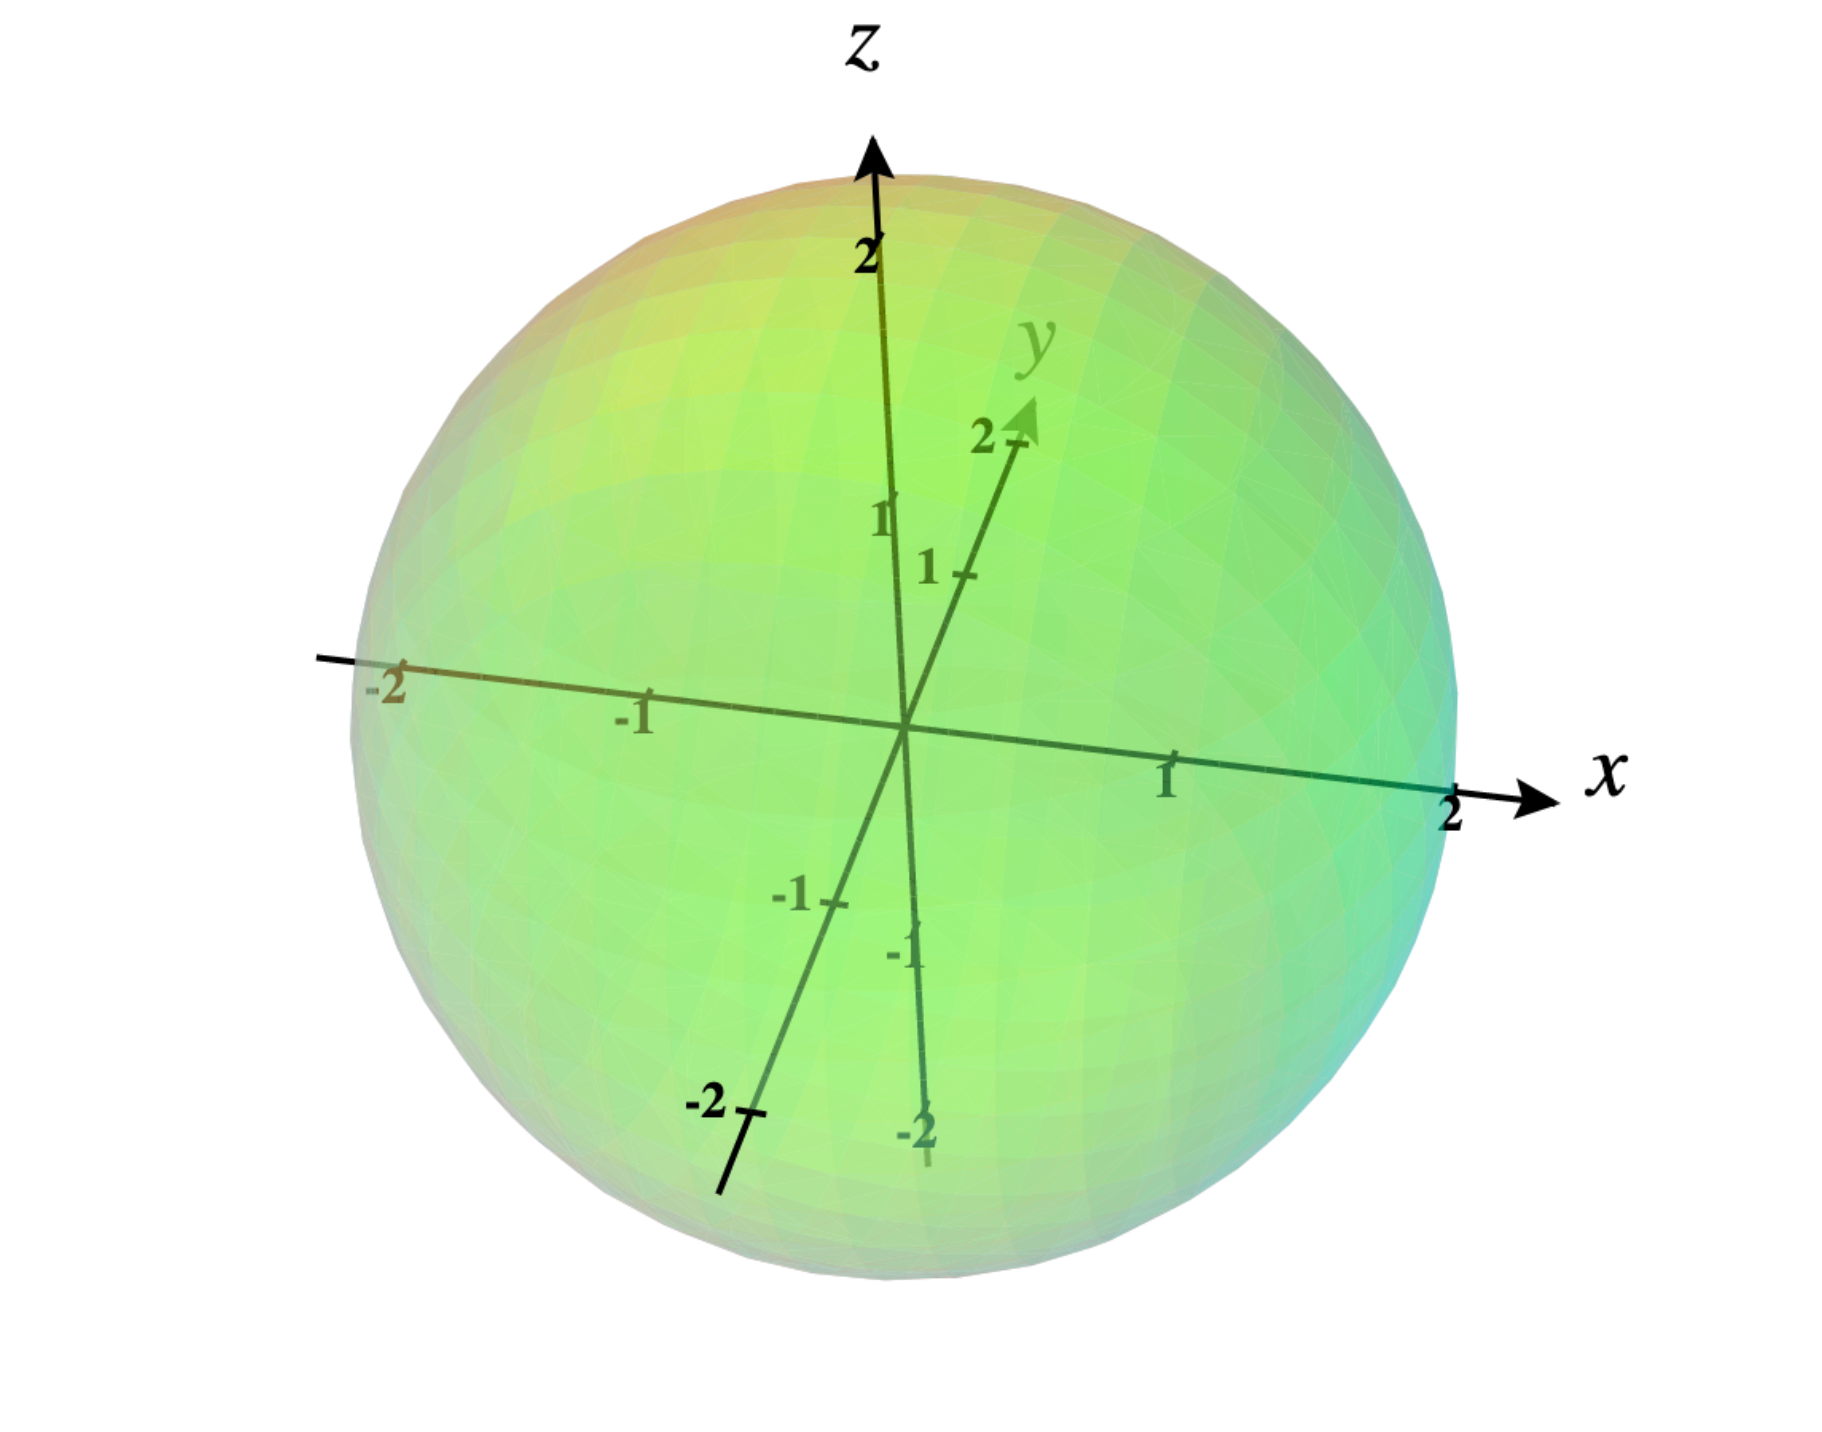
\includegraphics[width=.6\textwidth]{Images/level_surface_c0.png}
        \caption{Level surface for $h(x,y,z)=c_0$.}
    \end{figure}
        \begin{figure}[H]
        \centering
        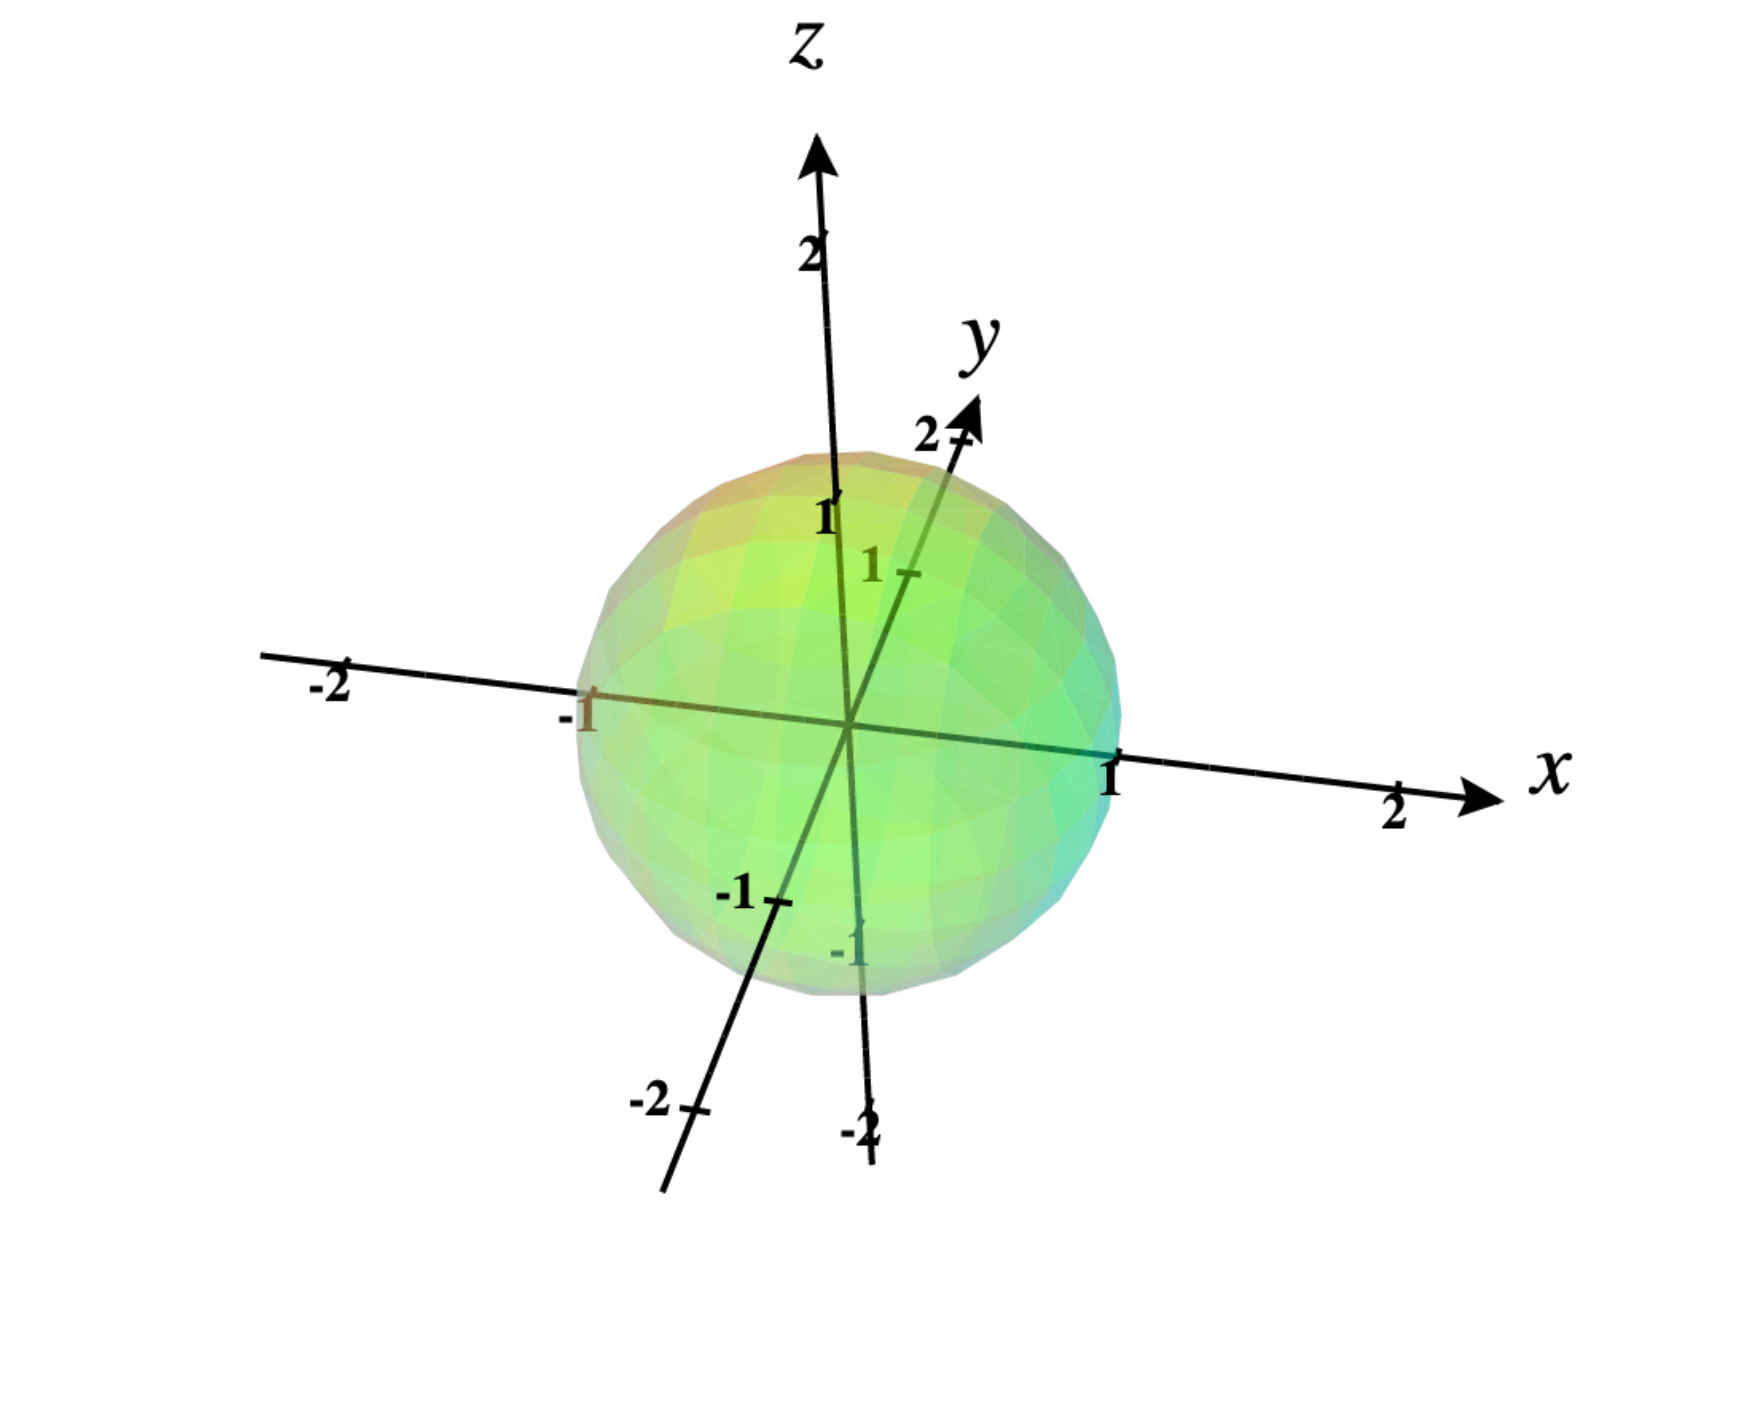
\includegraphics[width=.6\textwidth]{Images/level_surface_c1.png}
        \caption{Level surface for $h(x,y,z)=c_1$.}
    \end{figure}
        \begin{figure}[H]
        \centering
        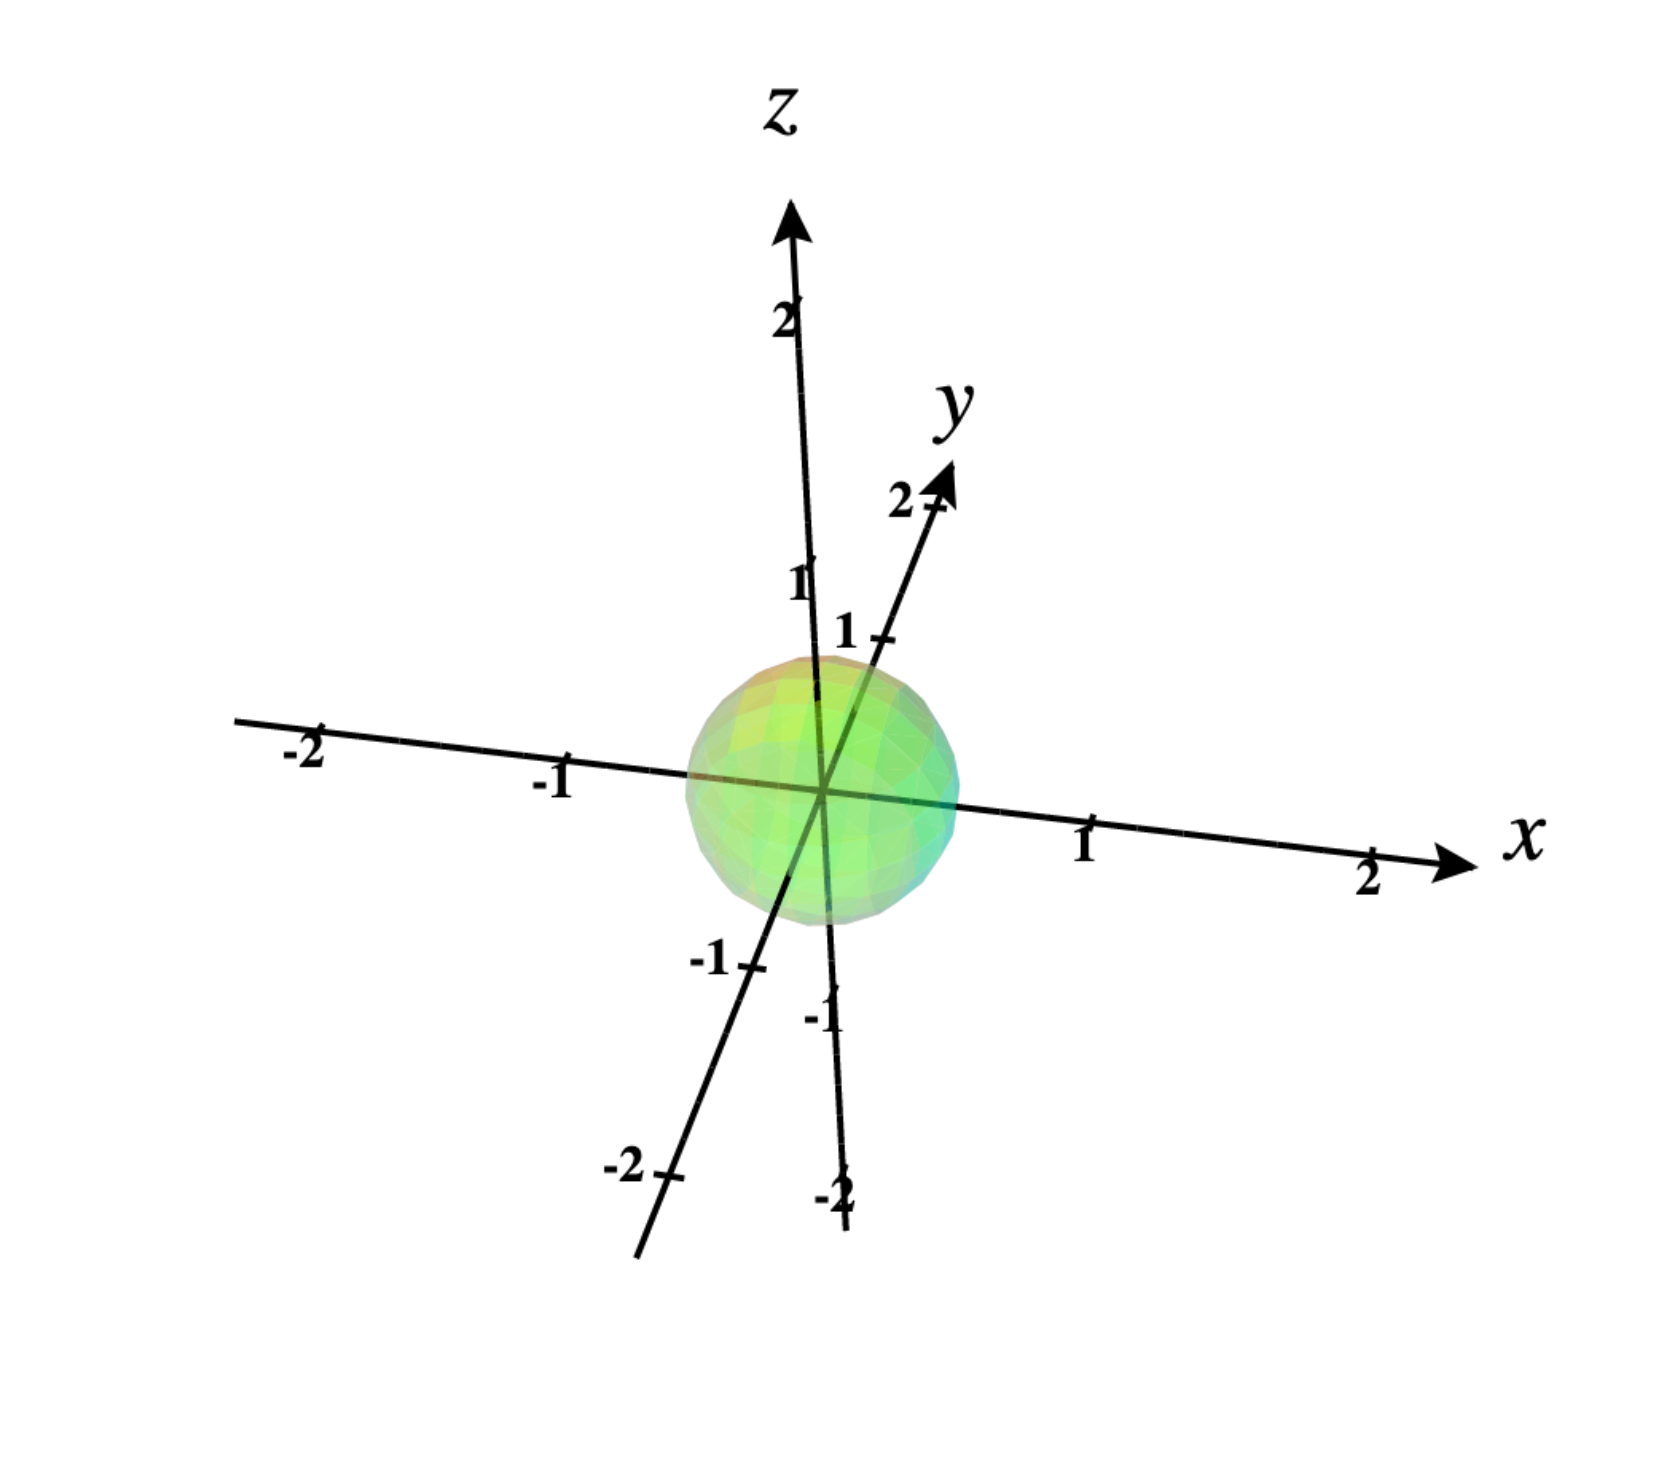
\includegraphics[width=.6\textwidth]{Images/level_surface_c2.png}
        \caption{Level surface for $h(x,y,z)=c_2$.}
    \end{figure}
        \begin{figure}[H]
        \centering
        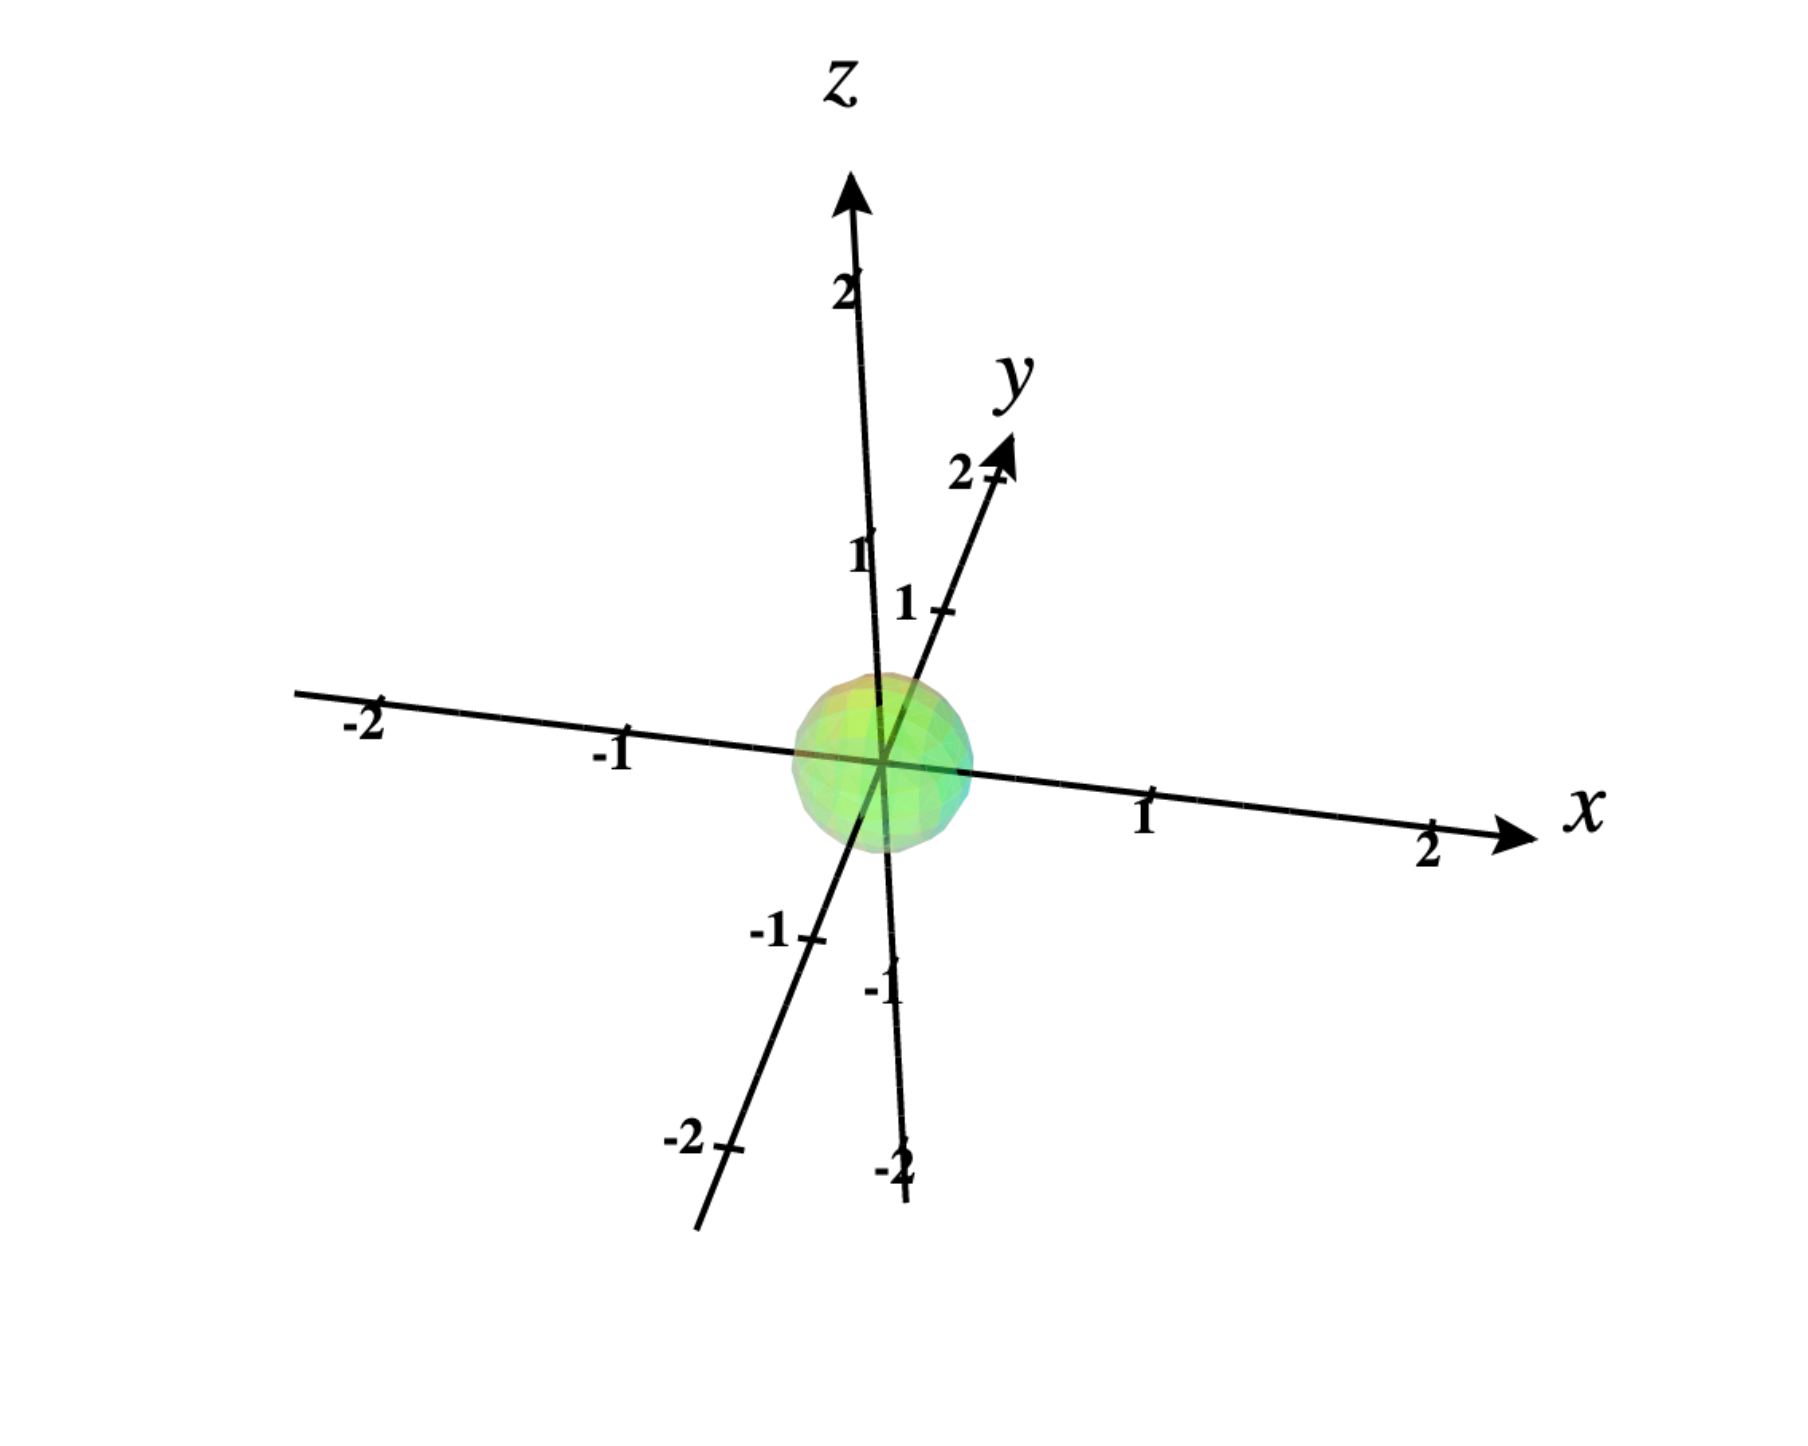
\includegraphics[width=.6\textwidth]{Images/level_surface_c3.png}
        \caption{Level surface for $h(x,y,z)=c_3$.}
    \end{figure}
\end{enumerate}
\end{solution}

\vspace*{.5cm}


\noindent\textbf{Problem 2.} Let
\[
f(x,y) = x^2+y^2-x^2y^2.
\]
\begin{enumerate}[(a)]
    \item Compute the equation for the tangent plane at the point $p=(1,2)$.
    \item Compute the gradient of $f$ and find the stationary point(s).
    \item Classify these point(s) as local maxima, local minima, or saddle points.
\end{enumerate}

\begin{solution}~
\begin{enumerate}[(a)]
    \item Let us compute the first partial derivatives
    \begin{align*}
        \frac{\partial f}{\partial x} &= 2x-2xy^2\\
        \frac{\partial f}{\partial y} &= 2y-2x^2y.
    \end{align*}
    Then we use the equation for the tangent plane
    \[
    z-f(x_0,y_0)= \left[ \frac{\partial f}{\partial x} \right]_{(x_0,y_0)} (x-x_0) + \left[\frac{\partial f}{\partial y} \right]_{(x_0,y_0)} (y-y_0),
    \]
    with $(x_0,y_0)=(1,2).$  So we have
    \begin{align*}
        z-f(1,2)&= \left[ \frac{\partial f}{\partial x}\right]_{(1,2)}(x-1)+\left[\frac{\partial f}{\partial y}\right]_{(1,2)}(y-2)\\
        z-1&= -6(x-1)+0(y-2).
    \end{align*}
    Here's a plot of this plane.
    \begin{figure}[H]
        \centering
        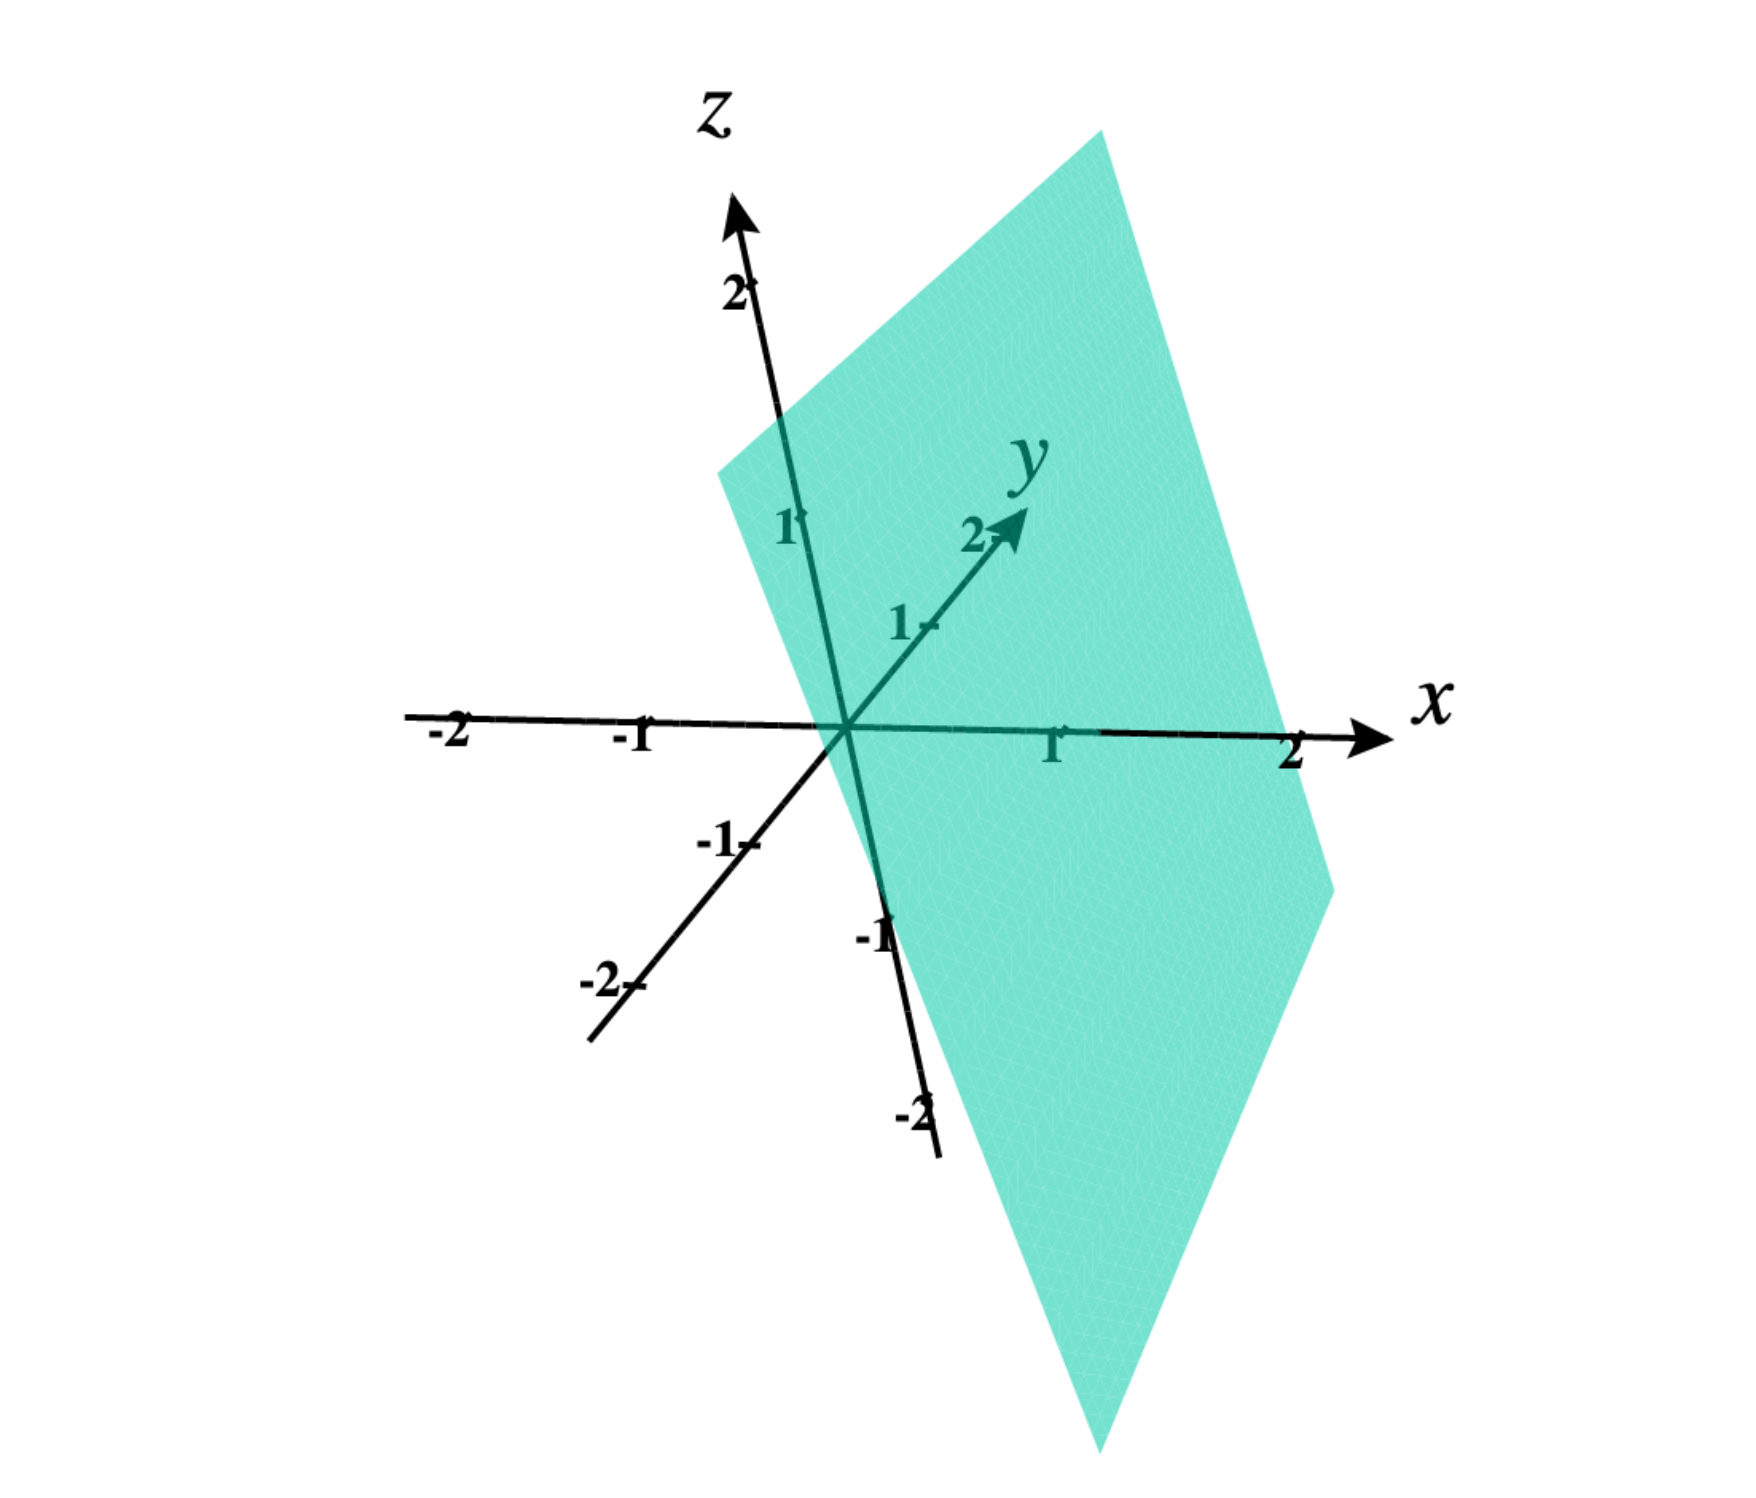
\includegraphics[width=.6\textwidth]{Images/tangent_plane.png}
    \end{figure}
    \item We already found the partial derivatives, so the gradient is
    \[
    \nabla f(x,y) = \begin{bmatrix} 2x-2xy^2 \\ 2y-2x^2y \end{bmatrix}.
    \]
    So to find stationary points we set this equal to zero, that is
    \begin{align*}
        \nabla f(x,y) = \mathbf{0}.
    \end{align*}
    This gives us the two equations
    \begin{align}
        2x-2xy^2 &= 0\\
        2y-2x^2y&=0,
    \end{align}
    for the two unknowns $x$ and $y$.
    
    Let us briefly look at the graph for this function.
    \begin{figure}[H]
        \centering
        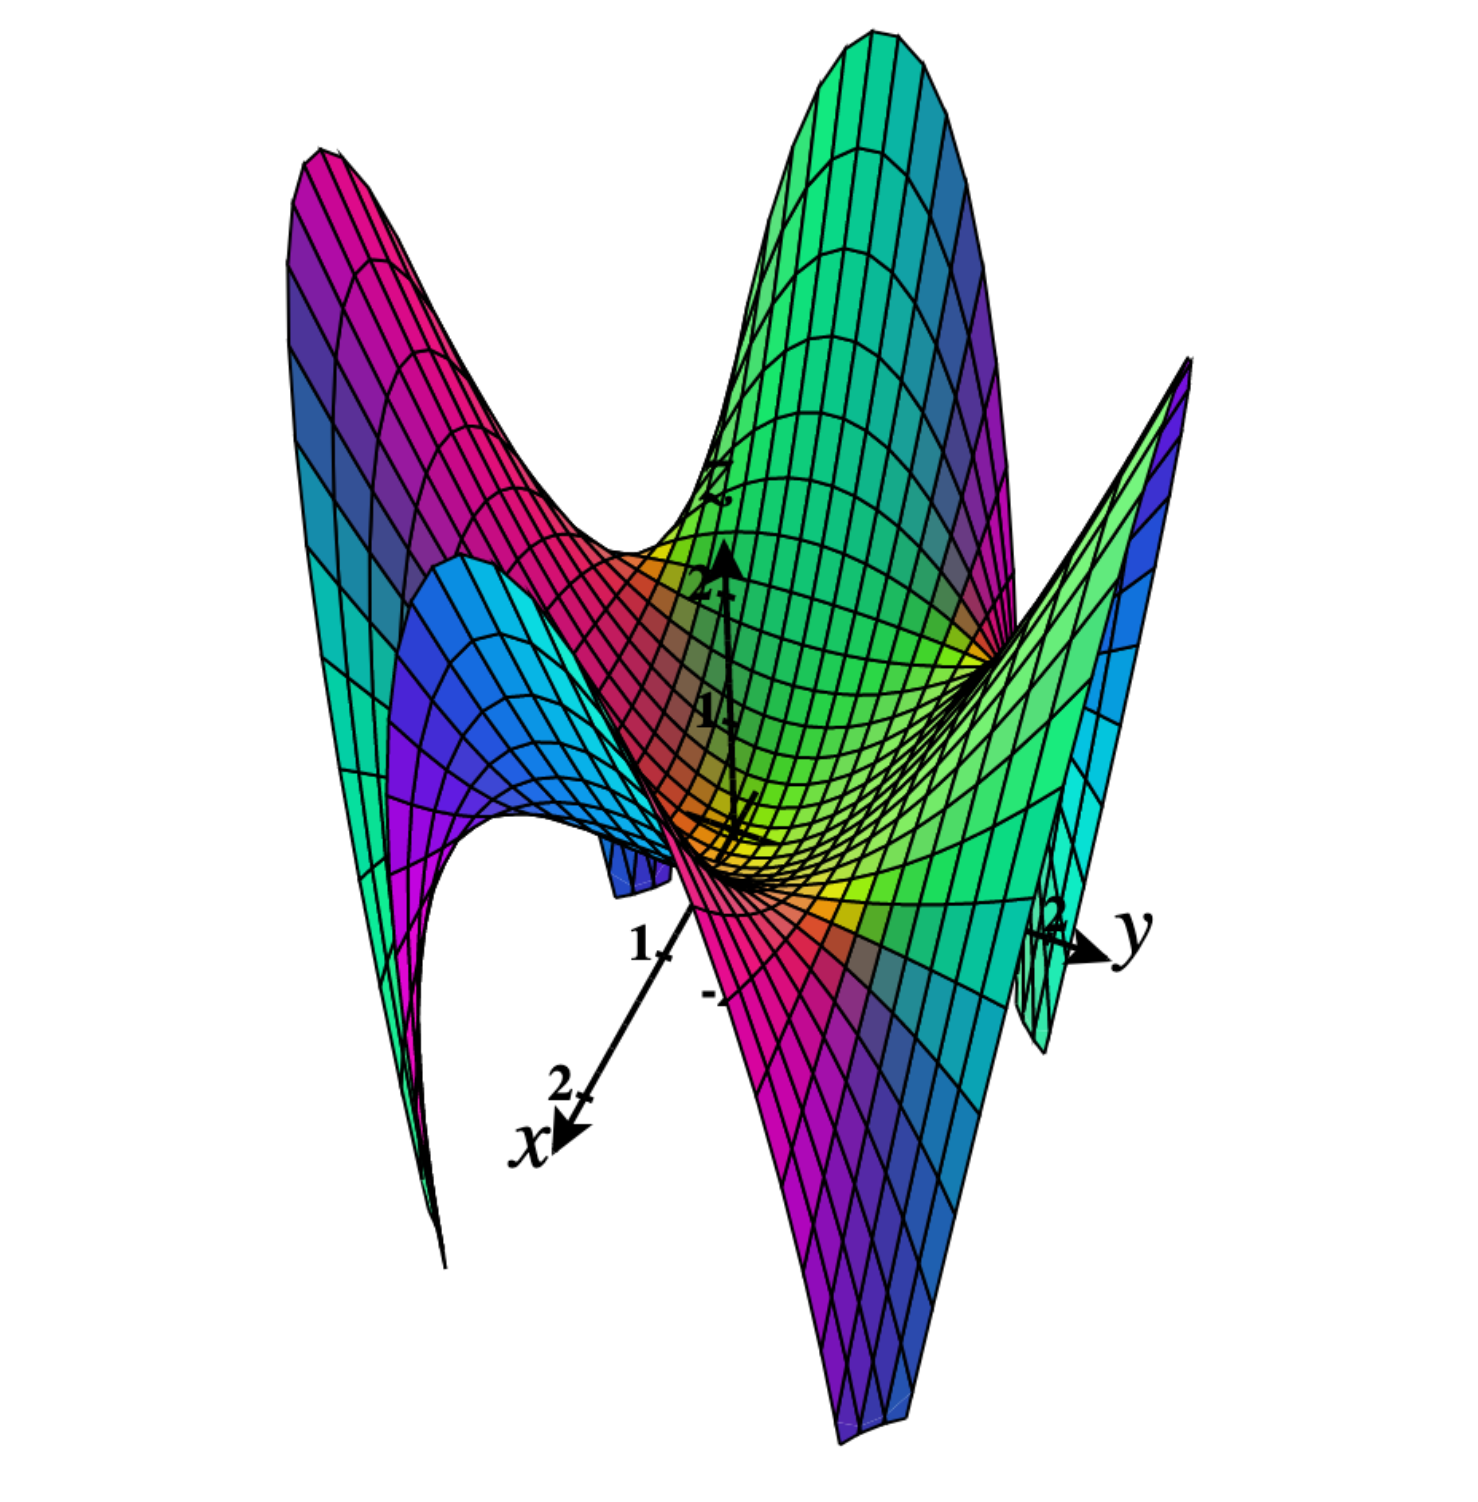
\includegraphics[width=.6\textwidth]{Images/stationary_point_surface.png}
    \end{figure}
    Notice that there are 4 saddle points and one minima.  So we expect 5 total stationary points.
\end{enumerate}
We can work with equation (1) first and find that it simplifies a bit
\[
2x(1-y^2)=0
\]
which means that this equation is zero when $x=0$ or $y=\pm 1$. Similarly, for (2) we have
\[
2y(1-x^2)=0
\]
which is zero for $y=0$ or $x=\pm 1$.

Using the information from (1), we take $x=0$ in equation (2) to see
\begin{align*}
    2y(1-0)&=0\\
    \iff 2y&=0
\end{align*}
which means $y=0$ also.  So one stationary point is $(0,0)$. Again, take $y=1$ from equation (1) and use this in (2)
\begin{align*}
    2(1)(1-x^2)&=0\\
    \iff x=\pm 1.
\end{align*}
So we found two new points, namely $(1,1)$ and $(-1,1)$.  Lastly, take $y=-1$ from equation (1) and use this in (2)
\begin{align*}
    2(-1)(1-x^2)&=0\\
    \iff x=\pm 1.
\end{align*}
Again, here are two new points $(1,-1)$ and $(-1,-1)$.  These are the 5 points we can see from the plot. There are no further points to be found since we have exhausted all possibilities from equation (1).
\item We should compute the second partial derivatives and then evaluate these at our points from before. So we have
\begin{align*}
    \frac{\partial ^2 f}{\partial x^2} &= 2-2y^2\\
    \frac{\partial^2 f}{\partial y^2} &= 2-2x^2.
\end{align*}
Then at each point,
\begin{align*}
    \textrm{For the point $(0,0)$:}&\quad \left[\frac{\partial^2 f}{\partial x^2}\right]_{(0,0)} = 2, ~ \left[\frac{\partial^2 f}{\partial y^2}\right]_{(0,0)} = 2 ~ \implies \textrm{minima},\\
    \textrm{For the point $(-1,-1)$:}&\quad \left[\frac{\partial^2 f}{\partial x^2}\right]_{(-1,-1)} = 0, ~ \left[\frac{\partial^2 f}{\partial y^2}\right]_{(-1,-1)} = 0 ~ \implies \textrm{saddle},\\
    \textrm{For the point $(-1,1)$:}&\quad \left[\frac{\partial^2 f}{\partial x^2}\right]_{(-1,1)} = 0, ~ \left[\frac{\partial^2 f}{\partial y^2}\right]_{(-1,1)} = 0 ~ \implies \textrm{saddle},\\
    \textrm{For the point $(1,-1)$:}&\quad \left[\frac{\partial^2 f}{\partial x^2}\right]_{(1,-1)} = 0, ~ \left[\frac{\partial^2 f}{\partial y^2}\right]_{(1,-1)} = 0 ~ \implies \textrm{saddle},\\
    \textrm{For the point $(1,1)$:}&\quad \left[\frac{\partial^2 f}{\partial x^2}\right]_{(1,1)} = 0, ~ \left[\frac{\partial^2 f}{\partial y^2}\right]_{(1,1)} = 0 ~ \implies \textrm{saddle}.
\end{align*}
Actually, the fact that the second partial derivatives are $0$ for the points $(-1,-1), (1,-1)$, $(-1,1), (1,1)$ does not quite tell us that these are saddle points.  However, the plot shows us that.  There is a way we can be a bit more careful about this,  but I did not go over that.  We can build a matrix of second derivatives called the \emph{Hessian} and the determinant of this matrix has a bit more information with it.
\end{solution}
\vspace*{.5cm}


\noindent\textbf{Problem 3.} Let
\[
\mathbf{v}(x,y,z)= ( x-y,y+x,z)
\]
be a vector field in $\R^3$.  
\begin{enumerate}[(a)]
    \item Find the Jacobian of this vector field. \emph{Note this quantity is a matrix!}
    \item Compute the determinant of the jacobian at the point $(0,0,0)$.  
    \item Write the component functions of $\mathbf{v}$ as follows:
    \begin{align*}
        v_1 (x,y,z) &= x-y,\\
        v_2(x,y,z) &= y+x,\\
        v_3(x,y,z) &= z.
    \end{align*}
    Compute the \emph{divergence} of $\mathbf{v}$
    \[
    \nabla \cdot \mathbf{v} \coloneqq \frac{\partial}{\partial x} v_1 + \frac{\partial}{\partial y} v_2 + \frac{\partial}{\partial z} v_3.
    \]
    \emph{Note this quantity is a scalar!}
    \item Compute the \emph{curl} of $\mathbf{v}$
    \[
    \nabla \times \mathbf{v} = \begin{bmatrix} \frac{\partial v_3}{\partial y} - \frac{\partial v_2}{\partial z} \\ \frac{\partial v_1}{\partial z} - \frac{\partial v_3}{\partial x} \\ \frac{\partial v_2}{\partial x} - \frac{\partial v_1}{\partial y} \end{bmatrix}
    \]
    \emph{Note this quantity is a vector!}
\end{enumerate}
\begin{solution}
\begin{enumerate}[(a)]
    \item We have that the Jacobian matrix is given by
    \[
    J(x,y,z) = \begin{bmatrix} \frac{\partial v_1}{\partial x} & \frac{\partial v_1}{\partial y} & \frac{\partial v_1}{\partial z} \\ 
    \frac{\partial v_2}{\partial x} & \frac{\partial v_2}{\partial y} & \frac{\partial v_2}{\partial z} \\
    \frac{\partial v_3}{\partial x} & \frac{\partial v_3}{\partial y} & \frac{\partial v_3}{\partial z} \end{bmatrix}.
    \]
    So we compute each partial and find
    \[
    J(x,y,z) = \begin{bmatrix} 1 & -1 & 0 \\ 1 & 1 & 0 \\ 0 & 0 & 1 \end{bmatrix}.
    \]
    \item It turns out this Jacobian is constant everywhere so evaluating the determinant is the same at every point.  We will find
    \[
    \det(J(0,0,0))= 2.
    \]
    Why is the Jacobian constant? It's because the vector field I gave you was linear! The Jacobian is the linearization of a vector field and if the field is already linear, then the Jacobian is constant.
    \item We have that
    \begin{align*}
        \frac{\partial}{\partial x} v_1 &=1\\
        \frac{\partial}{\partial y} v_2 &=1\\
        \frac{\partial}{\partial z} v_3 &=1.
    \end{align*}
    Of course, we computed these quantities before when computing the Jacobian. So it follows that
    \[
    \nabla \cdot \mathbf{v} = 1+1+1 = 3.
    \]
    \item We already computed all the necessary derivatives in the Jacobian, so I will just put the answer. We have
    \[
    \nabla \times \mathbf{v} = \begin{bmatrix} 0 \\ 0 \\ 2 \end{bmatrix}.
    \]
\end{enumerate}
\end{solution}
\vspace*{.5cm}



\noindent\textbf{*Problem 4.} Here we will use Lagrange multipliers to solve a constrained optimization problem.  In our case, we want to find where a function $f(x,y)$ is maximal and minimal when subject to a constraint function $g(x,y)$.  This type of problem is very common.  In fact, this is how we can show that the shape of a red blood cell is optimal for diffusion of oxygen for a given volume! The technique there is just a little bit more advanced.

For us, let's consider the function we want to optimize
\[
f(x,y,z)=xyz
\]
with the constraint 
\[
g(x,y,z)=x+y+z=1
\]
and $x,y,z\geq 0$. 

\emph{This is asking for what rectanglular prism with edges constructed from a given length of wire has the most volume. There will be a few options that you will have to check for which maximizes $f$.}
\begin{solution}
We wish to solve the set of equations
\begin{align*}
    \nabla f(x,y,z) &= \lambda \nabla g(x,y,z)\\
    g(x,y,z) &= 1.
\end{align*}
So we find
\begin{align*}
    \nabla f(x,y,z) &= \begin{bmatrix} yz \\ xz \\ xy \end{bmatrix}\\
    \nabla g(x,y,z) &= \begin{bmatrix} 1 \\ 1 \\ 1 \end{bmatrix}.
\end{align*}
So this gives us the equations
\begin{align}
    yz &= \lambda \\
    xz &= \lambda \\
    xy &= \lambda.
\end{align}
We can multiply (1) by $x$, (2) by $y$, and (3) by $z$ to get
\begin{align*}
    xyz&=\lambda x\\
    xyz&=\lambda y\\
    xyz&= \lambda z.
\end{align*}
This means that
\[
\lambda x = \lambda y = \lambda z
\]
and moreover that $x=y=z$. So we now use the constraint equation
\[
g(x,y,z)=x+y+z=1
\]
with $x=y=z$. Thus,
\[
x+x+x=3x=1 
\]
gives us that $x=y=z=\frac{1}{3}$.

\end{solution}
\vspace*{.5cm}

\noindent\textbf{Problem 5.} Now that we are handling functions of more variables, we need to integrate them.  Let's consider the functions
\[
T(x,y) = 1+ x+y
\]
which describes the temperature of a point in the $xy$-plane and
\[
C_p(x,y) = x^2+y^2.
\]
which tells us the \emph{heat capacity} of a point in the $xy$-plane. We can find the energy contained in a rectangular region $x_0\leq x \leq x_1$ and $y_0\leq y \leq y_1$ by
\[
E = \int_{y_0}^{y_1} \int_{x_0}^{x_1} T(x,y)C_p(x,y)dxdy.
\]
Find the energy in the square region $0 \leq x \leq 2$ and $0\leq y \leq 2$ for our given functions.
\begin{solution}
Let us first multiply
\[
T(x,y)C_p(x,y) = (1+x+y)(x^2+y^2)=x^3+x^2y+x^2+xy^2+y^3+y^2.
\]
So now we evaluate
\[
E=\int_0^2 \int_0^2 x^3+x^2y+x^2+xy^2+y^3+y^2 dx dy.
\]
So we get
\begin{align*}
    \int_0^2 \int_0^2 x^3+x^2y+x^2+xy^2+y^3+y^2 dx dy &= \int_0^2 2y^3+4y^2+\frac{8}{3}y+\frac{20}{3} dy\\
    &=\frac{112}{3}.
\end{align*}

\end{solution}






\end{document}  